\documentclass[twoside]{book}

% Packages required by doxygen
\usepackage{fixltx2e}
\usepackage{calc}
\usepackage{doxygen}
\usepackage[export]{adjustbox} % also loads graphicx
\usepackage{graphicx}
\usepackage[utf8]{inputenc}
\usepackage{makeidx}
\usepackage{multicol}
\usepackage{multirow}
\PassOptionsToPackage{warn}{textcomp}
\usepackage{textcomp}
\usepackage[nointegrals]{wasysym}
\usepackage[table]{xcolor}

% Font selection
\usepackage[T1]{fontenc}
\usepackage[scaled=.90]{helvet}
\usepackage{courier}
\usepackage{amssymb}
\usepackage{sectsty}
\renewcommand{\familydefault}{\sfdefault}
\allsectionsfont{%
  \fontseries{bc}\selectfont%
  \color{darkgray}%
}
\renewcommand{\DoxyLabelFont}{%
  \fontseries{bc}\selectfont%
  \color{darkgray}%
}
\newcommand{\+}{\discretionary{\mbox{\scriptsize$\hookleftarrow$}}{}{}}

% Page & text layout
\usepackage{geometry}
\geometry{%
  a4paper,%
  top=2.5cm,%
  bottom=2.5cm,%
  left=2.5cm,%
  right=2.5cm%
}
\tolerance=750
\hfuzz=15pt
\hbadness=750
\setlength{\emergencystretch}{15pt}
\setlength{\parindent}{0cm}
\setlength{\parskip}{3ex plus 2ex minus 2ex}
\makeatletter
\renewcommand{\paragraph}{%
  \@startsection{paragraph}{4}{0ex}{-1.0ex}{1.0ex}{%
    \normalfont\normalsize\bfseries\SS@parafont%
  }%
}
\renewcommand{\subparagraph}{%
  \@startsection{subparagraph}{5}{0ex}{-1.0ex}{1.0ex}{%
    \normalfont\normalsize\bfseries\SS@subparafont%
  }%
}
\makeatother

% Headers & footers
\usepackage{fancyhdr}
\pagestyle{fancyplain}
\fancyhead[LE]{\fancyplain{}{\bfseries\thepage}}
\fancyhead[CE]{\fancyplain{}{}}
\fancyhead[RE]{\fancyplain{}{\bfseries\leftmark}}
\fancyhead[LO]{\fancyplain{}{\bfseries\rightmark}}
\fancyhead[CO]{\fancyplain{}{}}
\fancyhead[RO]{\fancyplain{}{\bfseries\thepage}}
\fancyfoot[LE]{\fancyplain{}{}}
\fancyfoot[CE]{\fancyplain{}{}}
\fancyfoot[RE]{\fancyplain{}{\bfseries\scriptsize Generated by Doxygen }}
\fancyfoot[LO]{\fancyplain{}{\bfseries\scriptsize Generated by Doxygen }}
\fancyfoot[CO]{\fancyplain{}{}}
\fancyfoot[RO]{\fancyplain{}{}}
\renewcommand{\footrulewidth}{0.4pt}
\renewcommand{\chaptermark}[1]{%
  \markboth{#1}{}%
}
\renewcommand{\sectionmark}[1]{%
  \markright{\thesection\ #1}%
}

% Indices & bibliography
\usepackage{natbib}
\usepackage[titles]{tocloft}
\setcounter{tocdepth}{3}
\setcounter{secnumdepth}{5}
\makeindex

% Hyperlinks (required, but should be loaded last)
\usepackage{ifpdf}
\ifpdf
  \usepackage[pdftex,pagebackref=true]{hyperref}
\else
  \usepackage[ps2pdf,pagebackref=true]{hyperref}
\fi
\hypersetup{%
  colorlinks=true,%
  linkcolor=blue,%
  citecolor=blue,%
  unicode%
}

% Custom commands
\newcommand{\clearemptydoublepage}{%
  \newpage{\pagestyle{empty}\cleardoublepage}%
}

\usepackage{caption}
\captionsetup{labelsep=space,justification=centering,font={bf},singlelinecheck=off,skip=4pt,position=top}

%===== C O N T E N T S =====

\begin{document}

% Titlepage & ToC
\hypersetup{pageanchor=false,
             bookmarksnumbered=true,
             pdfencoding=unicode
            }
\pagenumbering{roman}
\begin{titlepage}
\vspace*{7cm}
\begin{center}%
{\Large 41012 }\\
\vspace*{1cm}
{\large Generated by Doxygen 1.8.11}\\
\end{center}
\end{titlepage}
\clearemptydoublepage
\tableofcontents
\clearemptydoublepage
\pagenumbering{arabic}
\hypersetup{pageanchor=true}

%--- Begin generated contents ---
\chapter{Assignment 2\+: Utilising Abstraction for a Range of Sensor Classes}
\label{index}\hypertarget{index}{}The program replicates two sensors, a laser and 2 radar sensors. The sensor will produce readings depending on their specifications and fuse the values depending on the method set, min, max or avg.\hypertarget{index_ac_doc_index_more_info}{}\section{Where to start}\label{index_ac_doc_index_more_info}

\begin{DoxyItemize}
\item This just divides the general instructions here for students
\end{DoxyItemize}\hypertarget{index_ac_doc_install}{}\section{Installation}\label{index_ac_doc_install}
\hypertarget{index_ac_doc_step1}{}\subsection{Step 1\+: Opening the box}\label{index_ac_doc_step1}
Openning the box\hypertarget{index_ac_doc_step2}{}\subsection{Step 2\+: Running applications}\label{index_ac_doc_step2}
The system needs three components running, please run\+:

\begin{DoxyVerb}./tests/controller_test ../cfg/sim.cfg
./tests/lo_up ../cfg/sim.cfg
./tests/acLoc ../cfg/sim.cfg\end{DoxyVerb}
 
\chapter{Bug List}
\label{bug}
\hypertarget{bug}{}

\begin{DoxyRefList}
\item[\label{bug__bug000001}%
\hypertarget{bug__bug000001}{}%
Class \hyperlink{classControl}{Control} ]none reported as of 2019-\/05-\/19 
\end{DoxyRefList}
\chapter{Hierarchical Index}
\section{Class Hierarchy}
This inheritance list is sorted roughly, but not completely, alphabetically\+:\begin{DoxyCompactList}
\item \contentsline{section}{Generator}{\pageref{classGenerator}}{}
\item \contentsline{section}{Ranger\+Fusion\+Interface}{\pageref{classRangerFusionInterface}}{}
\begin{DoxyCompactList}
\item \contentsline{section}{Ranger\+Fusion}{\pageref{classRangerFusion}}{}
\end{DoxyCompactList}
\item \contentsline{section}{Ranger\+Interface}{\pageref{classRangerInterface}}{}
\begin{DoxyCompactList}
\item \contentsline{section}{Ranger}{\pageref{classRanger}}{}
\begin{DoxyCompactList}
\item \contentsline{section}{Laser}{\pageref{classLaser}}{}
\item \contentsline{section}{Radar}{\pageref{classRadar}}{}
\end{DoxyCompactList}
\end{DoxyCompactList}
\end{DoxyCompactList}

\chapter{Class Index}
\section{Class List}
Here are the classes, structs, unions and interfaces with brief descriptions\+:\begin{DoxyCompactList}
\item\contentsline{section}{\hyperlink{classGenerator}{Generator} \\*Random Number \hyperlink{classGenerator}{Generator} }{\pageref{classGenerator}}{}
\item\contentsline{section}{\hyperlink{classLaser}{Laser} \\*\hyperlink{classLaser}{Laser} derived class of \hyperlink{classRanger}{Ranger} }{\pageref{classLaser}}{}
\item\contentsline{section}{\hyperlink{classRadar}{Radar} \\*\hyperlink{classRadar}{Radar} derived class of \hyperlink{classRanger}{Ranger} }{\pageref{classRadar}}{}
\item\contentsline{section}{\hyperlink{classRanger}{Ranger} \\*\hyperlink{classRanger}{Ranger} derived class of \hyperlink{classRanger}{Ranger} Interface }{\pageref{classRanger}}{}
\item\contentsline{section}{\hyperlink{classRangerFusion}{Ranger\+Fusion} \\*\hyperlink{classRangerFusion}{Ranger\+Fusion} derived class of \hyperlink{classRangerFusionInterface}{Ranger\+Fusion\+Interface} }{\pageref{classRangerFusion}}{}
\item\contentsline{section}{\hyperlink{classRangerFusionInterface}{Ranger\+Fusion\+Interface} \\*\hyperlink{classRangerFusionInterface}{Ranger\+Fusion\+Interface} base class }{\pageref{classRangerFusionInterface}}{}
\item\contentsline{section}{\hyperlink{classRangerInterface}{Ranger\+Interface} \\*\hyperlink{classRanger}{Ranger} interface base class }{\pageref{classRangerInterface}}{}
\end{DoxyCompactList}

\chapter{Class Documentation}
\hypertarget{classGenerator}{}\section{Generator Class Reference}
\label{classGenerator}\index{Generator@{Generator}}


Random Number \hyperlink{classGenerator}{Generator}.  




{\ttfamily \#include $<$generator.\+h$>$}

\subsection*{Public Member Functions}
\begin{DoxyCompactItemize}
\item 
\hyperlink{classGenerator_a14b6bb40fe312824f6ab882336fa53ac}{Generator} (int seed)\hypertarget{classGenerator_a14b6bb40fe312824f6ab882336fa53ac}{}\label{classGenerator_a14b6bb40fe312824f6ab882336fa53ac}

\begin{DoxyCompactList}\small\item\em Takes a seed for random values. \end{DoxyCompactList}\item 
double \hyperlink{classGenerator_a6d2596bcce1864d629484739acddde9f}{Random\+Numbers} (double mean, double std\+Dev, double max)
\end{DoxyCompactItemize}


\subsection{Detailed Description}
Random Number \hyperlink{classGenerator}{Generator}. 

This is the random number generator class.~\newline
\begin{DoxyAuthor}{Author}
Johnsonn Nguyen 
\end{DoxyAuthor}
\begin{DoxyVersion}{Version}
1 
\end{DoxyVersion}
\begin{DoxyDate}{Date}
2019 
\end{DoxyDate}
\begin{DoxyPrecond}{Precondition}
none 
\end{DoxyPrecond}
\begin{DoxyRefDesc}{Bug}
\item[\hyperlink{bug__bug000001}{Bug}]none reported as of 2019-\/04-\/23 \end{DoxyRefDesc}
\begin{DoxyWarning}{Warning}

\end{DoxyWarning}


\subsection{Member Function Documentation}
\index{Generator@{Generator}!Random\+Numbers@{Random\+Numbers}}
\index{Random\+Numbers@{Random\+Numbers}!Generator@{Generator}}
\subsubsection[{\texorpdfstring{Random\+Numbers(double mean, double std\+Dev, double max)}{RandomNumbers(double mean, double stdDev, double max)}}]{\setlength{\rightskip}{0pt plus 5cm}double Generator\+::\+Random\+Numbers (
\begin{DoxyParamCaption}
\item[{double}]{mean, }
\item[{double}]{std\+Dev, }
\item[{double}]{max}
\end{DoxyParamCaption}
)}\hypertarget{classGenerator_a6d2596bcce1864d629484739acddde9f}{}\label{classGenerator_a6d2596bcce1864d629484739acddde9f}
takes the mean, standard deviation and max value returns the random number 

The documentation for this class was generated from the following files\+:\begin{DoxyCompactItemize}
\item 
/home/user/git/pfms-\/2019a-\/\+Johnson15177/scratch/assignment/a2attempt2/generator.\+h\item 
/home/user/git/pfms-\/2019a-\/\+Johnson15177/scratch/assignment/a2attempt2/generator.\+cpp\end{DoxyCompactItemize}

\hypertarget{classLaser}{}\section{Laser Class Reference}
\label{classLaser}\index{Laser@{Laser}}


\hyperlink{classLaser}{Laser} derived class of \hyperlink{classRanger}{Ranger}.  




{\ttfamily \#include $<$laser.\+h$>$}

Inheritance diagram for Laser\+:\begin{figure}[H]
\begin{center}
\leavevmode
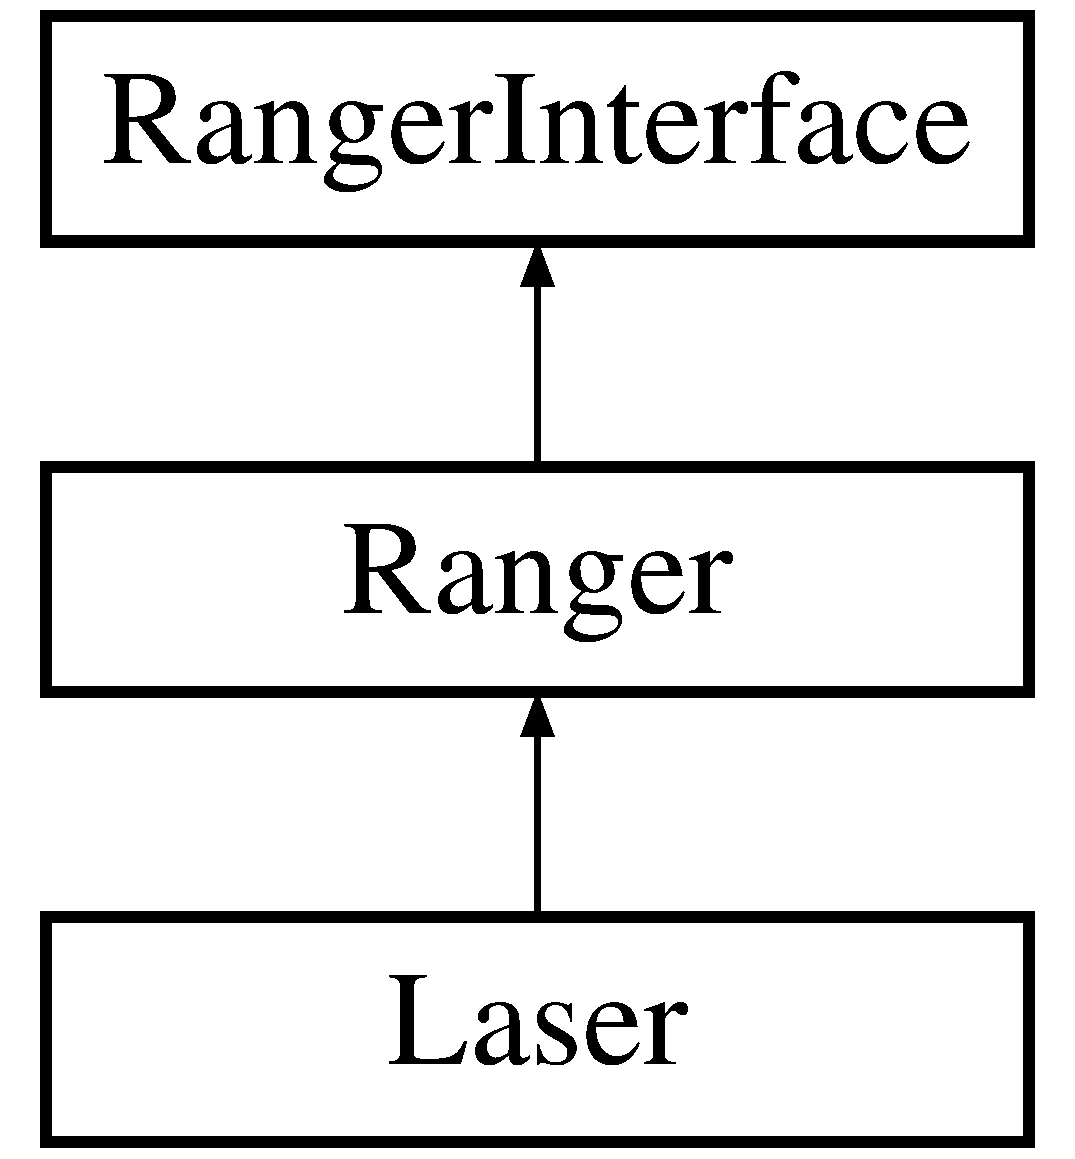
\includegraphics[height=3.000000cm]{classLaser}
\end{center}
\end{figure}
\subsection*{Public Member Functions}
\begin{DoxyCompactItemize}
\item 
vector$<$ double $>$ \hyperlink{classLaser_af5345ed85a07caa86c52b19d7eff738e}{generate\+Data} ()\hypertarget{classLaser_af5345ed85a07caa86c52b19d7eff738e}{}\label{classLaser_af5345ed85a07caa86c52b19d7eff738e}

\begin{DoxyCompactList}\small\item\em generates data depending on the F\+OV and angular resolution for laser \end{DoxyCompactList}\item 
string \hyperlink{classLaser_ae0d6251839324eb65a7c06605a79adf2}{get\+Model} (void)\hypertarget{classLaser_ae0d6251839324eb65a7c06605a79adf2}{}\label{classLaser_ae0d6251839324eb65a7c06605a79adf2}

\begin{DoxyCompactList}\small\item\em gets the string of the model for laser \end{DoxyCompactList}\item 
unsigned int \hyperlink{classLaser_a65ef9cdae59880120965e4a2ae9a927f}{get\+Field\+Of\+View} (void)\hypertarget{classLaser_a65ef9cdae59880120965e4a2ae9a927f}{}\label{classLaser_a65ef9cdae59880120965e4a2ae9a927f}

\begin{DoxyCompactList}\small\item\em gets the field of view for laser \end{DoxyCompactList}\item 
unsigned int \hyperlink{classLaser_a8cca3c1ff26bd1c021017bda97bd32be}{get\+Angular\+Resolution} (void)\hypertarget{classLaser_a8cca3c1ff26bd1c021017bda97bd32be}{}\label{classLaser_a8cca3c1ff26bd1c021017bda97bd32be}

\begin{DoxyCompactList}\small\item\em gets the angular resolution for laser \end{DoxyCompactList}\item 
int \hyperlink{classLaser_a68d52b516007a7762b5089913e7d6a5b}{get\+Offset} (void)\hypertarget{classLaser_a68d52b516007a7762b5089913e7d6a5b}{}\label{classLaser_a68d52b516007a7762b5089913e7d6a5b}

\begin{DoxyCompactList}\small\item\em gets the offset for laser \end{DoxyCompactList}\item 
bool \hyperlink{classLaser_a972cefe67bc16f5e781f7a91bdf5bbea}{set\+Field\+Of\+View} (unsigned int)\hypertarget{classLaser_a972cefe67bc16f5e781f7a91bdf5bbea}{}\label{classLaser_a972cefe67bc16f5e781f7a91bdf5bbea}

\begin{DoxyCompactList}\small\item\em sets the field of view for laser \end{DoxyCompactList}\item 
bool \hyperlink{classLaser_a67c6742c5854f3d0476a1267c86b44e8}{set\+Angular\+Resolution} (unsigned int)\hypertarget{classLaser_a67c6742c5854f3d0476a1267c86b44e8}{}\label{classLaser_a67c6742c5854f3d0476a1267c86b44e8}

\begin{DoxyCompactList}\small\item\em sets the angular resolution for laser \end{DoxyCompactList}\item 
bool \hyperlink{classLaser_af0fe35dc98cf26a2bd2eaebcba55a406}{set\+Offset} (int)\hypertarget{classLaser_af0fe35dc98cf26a2bd2eaebcba55a406}{}\label{classLaser_af0fe35dc98cf26a2bd2eaebcba55a406}

\begin{DoxyCompactList}\small\item\em sets the offset for laser \end{DoxyCompactList}\item 
double \hyperlink{classLaser_a60e9bba1da9aea6058e281c4d0f545cc}{get\+Min\+Range} (void)\hypertarget{classLaser_a60e9bba1da9aea6058e281c4d0f545cc}{}\label{classLaser_a60e9bba1da9aea6058e281c4d0f545cc}

\begin{DoxyCompactList}\small\item\em gets the min range for laser \end{DoxyCompactList}\item 
double \hyperlink{classLaser_a85990956d2a5aea589a47e1a9989c4ce}{get\+Max\+Range} (void)\hypertarget{classLaser_a85990956d2a5aea589a47e1a9989c4ce}{}\label{classLaser_a85990956d2a5aea589a47e1a9989c4ce}

\begin{DoxyCompactList}\small\item\em gets the max range for laser \end{DoxyCompactList}\end{DoxyCompactItemize}


\subsection{Detailed Description}
\hyperlink{classLaser}{Laser} derived class of \hyperlink{classRanger}{Ranger}. 

This is the derived class of \hyperlink{classRanger}{Ranger}.~\newline
\begin{DoxyAuthor}{Author}
Johnsonn Nguyen 
\end{DoxyAuthor}
\begin{DoxyVersion}{Version}
1 
\end{DoxyVersion}
\begin{DoxyDate}{Date}
2019 
\end{DoxyDate}
\begin{DoxyPrecond}{Precondition}
none 
\end{DoxyPrecond}
\begin{DoxyRefDesc}{Bug}
\item[\hyperlink{bug__bug000002}{Bug}]none reported as of 2019-\/04-\/23 \end{DoxyRefDesc}
\begin{DoxyWarning}{Warning}

\end{DoxyWarning}


The documentation for this class was generated from the following files\+:\begin{DoxyCompactItemize}
\item 
/home/user/git/pfms-\/2019a-\/\+Johnson15177/scratch/assignment/a2attempt2/laser.\+h\item 
/home/user/git/pfms-\/2019a-\/\+Johnson15177/scratch/assignment/a2attempt2/laser.\+cpp\end{DoxyCompactItemize}

\hypertarget{classRadar}{}\section{Radar Class Reference}
\label{classRadar}\index{Radar@{Radar}}


\hyperlink{classRadar}{Radar} derived class of \hyperlink{classRanger}{Ranger}.  




{\ttfamily \#include $<$radar.\+h$>$}

Inheritance diagram for Radar\+:\begin{figure}[H]
\begin{center}
\leavevmode
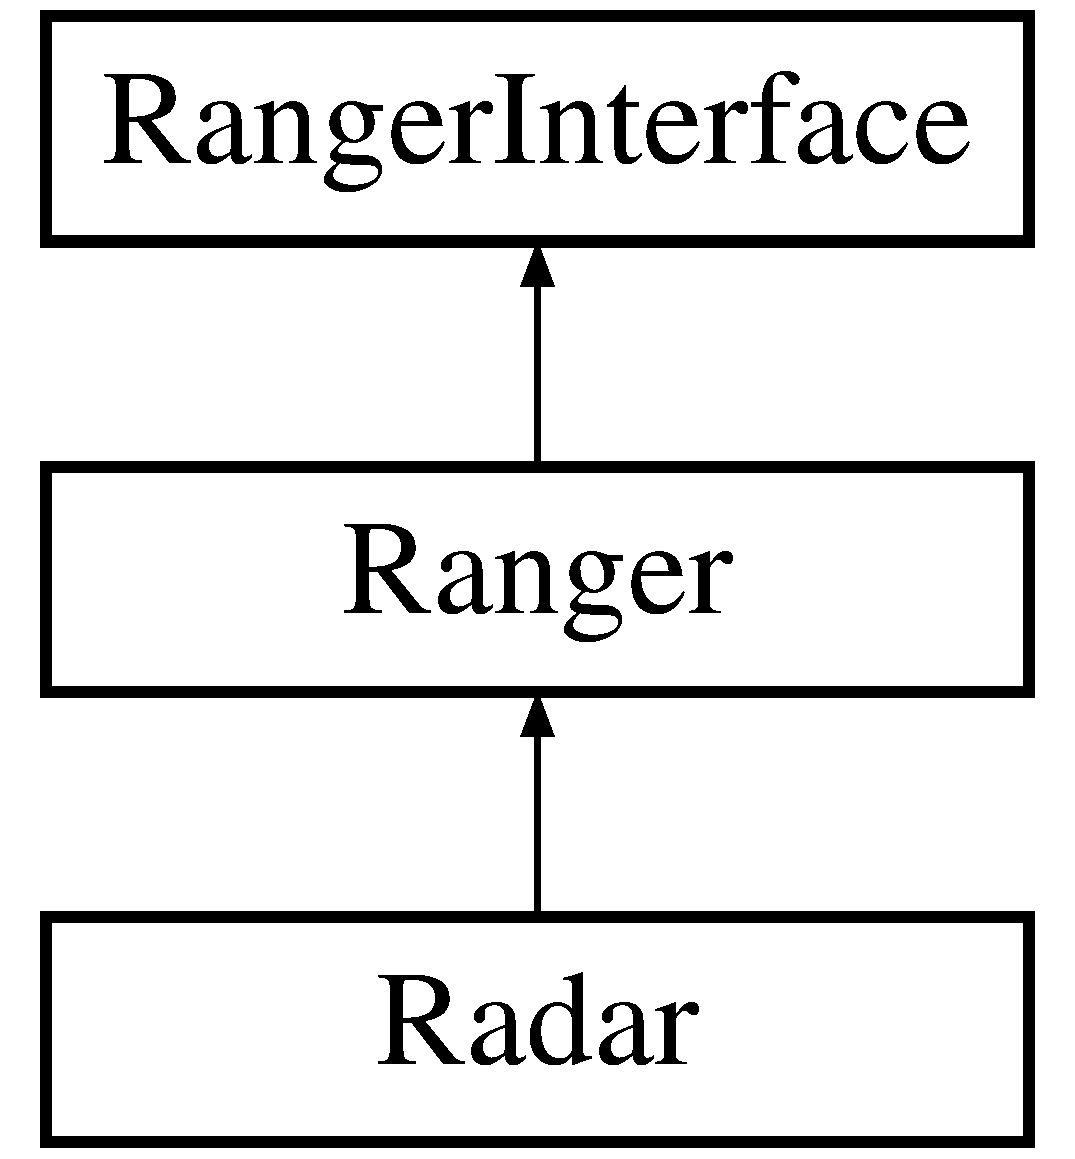
\includegraphics[height=3.000000cm]{classRadar}
\end{center}
\end{figure}
\subsection*{Public Member Functions}
\begin{DoxyCompactItemize}
\item 
vector$<$ double $>$ \hyperlink{classRadar_a45ac8b0ad39dd402706e52733c8d372f}{generate\+Data} ()\hypertarget{classRadar_a45ac8b0ad39dd402706e52733c8d372f}{}\label{classRadar_a45ac8b0ad39dd402706e52733c8d372f}

\begin{DoxyCompactList}\small\item\em generates data depending on the F\+OV and angular resolution for radar \end{DoxyCompactList}\item 
string \hyperlink{classRadar_a95997166ffc91d1af644b0dcf2b7a80c}{get\+Model} (void)\hypertarget{classRadar_a95997166ffc91d1af644b0dcf2b7a80c}{}\label{classRadar_a95997166ffc91d1af644b0dcf2b7a80c}

\begin{DoxyCompactList}\small\item\em gets the string of the model for radar \end{DoxyCompactList}\item 
unsigned int \hyperlink{classRadar_a775fbd0f15b61d51d071f4e9c0305113}{get\+Field\+Of\+View} (void)\hypertarget{classRadar_a775fbd0f15b61d51d071f4e9c0305113}{}\label{classRadar_a775fbd0f15b61d51d071f4e9c0305113}

\begin{DoxyCompactList}\small\item\em gets the field of view for radar \end{DoxyCompactList}\item 
unsigned int \hyperlink{classRadar_a8253881e17e63ef80945b2c472189c9d}{get\+Angular\+Resolution} (void)\hypertarget{classRadar_a8253881e17e63ef80945b2c472189c9d}{}\label{classRadar_a8253881e17e63ef80945b2c472189c9d}

\begin{DoxyCompactList}\small\item\em gets the angular resolution for radar \end{DoxyCompactList}\item 
int \hyperlink{classRadar_adb5af48c1858d3d3e064cb104ad04890}{get\+Offset} (void)\hypertarget{classRadar_adb5af48c1858d3d3e064cb104ad04890}{}\label{classRadar_adb5af48c1858d3d3e064cb104ad04890}

\begin{DoxyCompactList}\small\item\em gets the offset for radar \end{DoxyCompactList}\item 
bool \hyperlink{classRadar_a1a178ebacc58825322a127b9c4565202}{set\+Field\+Of\+View} (unsigned int)\hypertarget{classRadar_a1a178ebacc58825322a127b9c4565202}{}\label{classRadar_a1a178ebacc58825322a127b9c4565202}

\begin{DoxyCompactList}\small\item\em sets the field of view for radar \end{DoxyCompactList}\item 
bool \hyperlink{classRadar_ad2033a6eed26d66446a52222cc6c7440}{set\+Angular\+Resolution} (unsigned int)\hypertarget{classRadar_ad2033a6eed26d66446a52222cc6c7440}{}\label{classRadar_ad2033a6eed26d66446a52222cc6c7440}

\begin{DoxyCompactList}\small\item\em sets the angular resolution for radar \end{DoxyCompactList}\item 
bool \hyperlink{classRadar_adb2141cd70f71326034fd5f555222f7a}{set\+Offset} (int)\hypertarget{classRadar_adb2141cd70f71326034fd5f555222f7a}{}\label{classRadar_adb2141cd70f71326034fd5f555222f7a}

\begin{DoxyCompactList}\small\item\em sets the offset for radar \end{DoxyCompactList}\item 
double \hyperlink{classRadar_a27e531152e4e4602226b1a6831b19d50}{get\+Min\+Range} (void)\hypertarget{classRadar_a27e531152e4e4602226b1a6831b19d50}{}\label{classRadar_a27e531152e4e4602226b1a6831b19d50}

\begin{DoxyCompactList}\small\item\em gets the min range for radar \end{DoxyCompactList}\item 
double \hyperlink{classRadar_a08fb7eae931cf82b24135230bbded208}{get\+Max\+Range} (void)\hypertarget{classRadar_a08fb7eae931cf82b24135230bbded208}{}\label{classRadar_a08fb7eae931cf82b24135230bbded208}

\begin{DoxyCompactList}\small\item\em gets the max range for radar \end{DoxyCompactList}\end{DoxyCompactItemize}


\subsection{Detailed Description}
\hyperlink{classRadar}{Radar} derived class of \hyperlink{classRanger}{Ranger}. 

This is the derived class of \hyperlink{classRanger}{Ranger}.~\newline
\begin{DoxyAuthor}{Author}
Johnsonn Nguyen 
\end{DoxyAuthor}
\begin{DoxyVersion}{Version}
1 
\end{DoxyVersion}
\begin{DoxyDate}{Date}
2019 
\end{DoxyDate}
\begin{DoxyPrecond}{Precondition}
none 
\end{DoxyPrecond}
\begin{DoxyRefDesc}{Bug}
\item[\hyperlink{bug__bug000003}{Bug}]none reported as of 2019-\/04-\/23 \end{DoxyRefDesc}
\begin{DoxyWarning}{Warning}

\end{DoxyWarning}


The documentation for this class was generated from the following files\+:\begin{DoxyCompactItemize}
\item 
/home/user/git/pfms-\/2019a-\/\+Johnson15177/scratch/assignment/a2attempt2/radar.\+h\item 
/home/user/git/pfms-\/2019a-\/\+Johnson15177/scratch/assignment/a2attempt2/radar.\+cpp\end{DoxyCompactItemize}

\hypertarget{classRanger}{}\section{Ranger Class Reference}
\label{classRanger}\index{Ranger@{Ranger}}


\hyperlink{classRanger}{Ranger} derived class of \hyperlink{classRanger}{Ranger} Interface.  




{\ttfamily \#include $<$ranger.\+h$>$}

Inheritance diagram for Ranger\+:\begin{figure}[H]
\begin{center}
\leavevmode
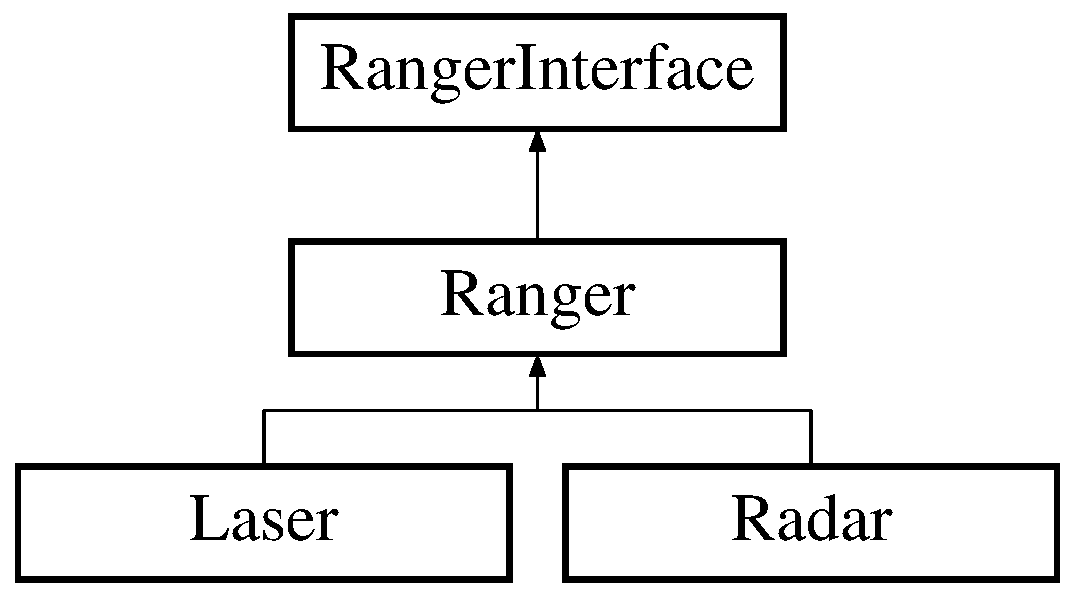
\includegraphics[height=3.000000cm]{classRanger}
\end{center}
\end{figure}
\subsection*{Public Member Functions}
\begin{DoxyCompactItemize}
\item 
virtual string \hyperlink{classRanger_aeac655d8f4543a8fc7218de555882fd4}{get\+Model} (void)=0\hypertarget{classRanger_aeac655d8f4543a8fc7218de555882fd4}{}\label{classRanger_aeac655d8f4543a8fc7218de555882fd4}

\begin{DoxyCompactList}\small\item\em gets the model for laser and radar \end{DoxyCompactList}\end{DoxyCompactItemize}


\subsection{Detailed Description}
\hyperlink{classRanger}{Ranger} derived class of \hyperlink{classRanger}{Ranger} Interface. 

This is the derived class of \hyperlink{classRanger}{Ranger} Interface.~\newline
\begin{DoxyAuthor}{Author}
Johnsonn Nguyen 
\end{DoxyAuthor}
\begin{DoxyVersion}{Version}
1 
\end{DoxyVersion}
\begin{DoxyDate}{Date}
2019 
\end{DoxyDate}
\begin{DoxyPrecond}{Precondition}
none 
\end{DoxyPrecond}
\begin{DoxyRefDesc}{Bug}
\item[\hyperlink{bug__bug000004}{Bug}]none reported as of 2019-\/04-\/23 \end{DoxyRefDesc}
\begin{DoxyWarning}{Warning}

\end{DoxyWarning}


The documentation for this class was generated from the following files\+:\begin{DoxyCompactItemize}
\item 
/home/user/git/pfms-\/2019a-\/\+Johnson15177/scratch/assignment/a2attempt2/ranger.\+h\item 
/home/user/git/pfms-\/2019a-\/\+Johnson15177/scratch/assignment/a2attempt2/ranger.\+cpp\end{DoxyCompactItemize}

\hypertarget{classRangerFusion}{}\section{Ranger\+Fusion Class Reference}
\label{classRangerFusion}\index{Ranger\+Fusion@{Ranger\+Fusion}}


\hyperlink{classRangerFusion}{Ranger\+Fusion} derived class of \hyperlink{classRangerFusionInterface}{Ranger\+Fusion\+Interface}.  




{\ttfamily \#include $<$rangerfusion.\+h$>$}

Inheritance diagram for Ranger\+Fusion\+:\begin{figure}[H]
\begin{center}
\leavevmode
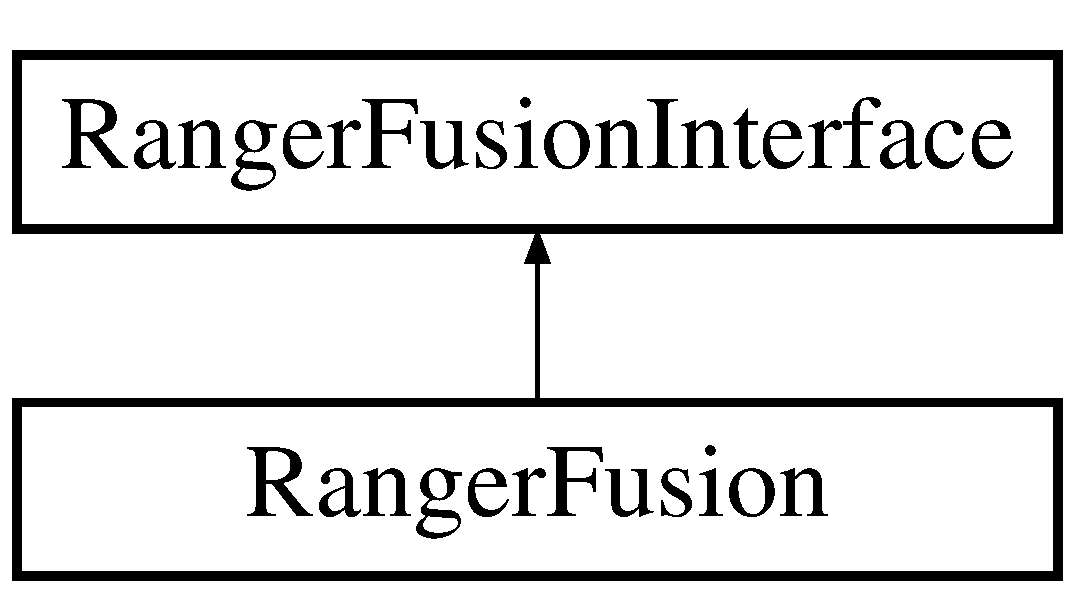
\includegraphics[height=2.000000cm]{classRangerFusion}
\end{center}
\end{figure}
\subsection*{Public Member Functions}
\begin{DoxyCompactItemize}
\item 
void \hyperlink{classRangerFusion_a01909c08b2a974e68b031056db730aba}{set\+Rangers} (std\+::vector$<$ \hyperlink{classRangerInterface}{Ranger\+Interface} $\ast$ $>$ rangers)\hypertarget{classRangerFusion_a01909c08b2a974e68b031056db730aba}{}\label{classRangerFusion_a01909c08b2a974e68b031056db730aba}

\begin{DoxyCompactList}\small\item\em stores the sensor objects inside the vector \end{DoxyCompactList}\item 
std\+::vector$<$ std\+::vector$<$ double $>$ $>$ \hyperlink{classRangerFusion_a5780383fdffe121a7a2372a047819ba9}{get\+Raw\+Range\+Data} ()\hypertarget{classRangerFusion_a5780383fdffe121a7a2372a047819ba9}{}\label{classRangerFusion_a5780383fdffe121a7a2372a047819ba9}

\begin{DoxyCompactList}\small\item\em generates the data for each sensor and the fused vector as well \end{DoxyCompactList}\item 
std\+::vector$<$ double $>$ \hyperlink{classRangerFusion_a2d68f0291653a422603ea9c8f2e33c21}{get\+Fused\+Range\+Data} ()\hypertarget{classRangerFusion_a2d68f0291653a422603ea9c8f2e33c21}{}\label{classRangerFusion_a2d68f0291653a422603ea9c8f2e33c21}

\begin{DoxyCompactList}\small\item\em returns the fused vector \end{DoxyCompactList}\item 
void \hyperlink{classRangerFusion_a1fc8c1b4a4e07225a2d51bc444ce049f}{set\+Fusion\+Method} (Fusion\+Method)\hypertarget{classRangerFusion_a1fc8c1b4a4e07225a2d51bc444ce049f}{}\label{classRangerFusion_a1fc8c1b4a4e07225a2d51bc444ce049f}

\begin{DoxyCompactList}\small\item\em provides calculations of each method of min, max and average, replaces fused vector with values depending on the method chosen \end{DoxyCompactList}\item 
bool \hyperlink{classRangerFusion_a49b3a2346c2d047274a3ad445a05b66f}{take\+Input} (unsigned int input)\hypertarget{classRangerFusion_a49b3a2346c2d047274a3ad445a05b66f}{}\label{classRangerFusion_a49b3a2346c2d047274a3ad445a05b66f}

\begin{DoxyCompactList}\small\item\em sets the method to be used \end{DoxyCompactList}\end{DoxyCompactItemize}


\subsection{Detailed Description}
\hyperlink{classRangerFusion}{Ranger\+Fusion} derived class of \hyperlink{classRangerFusionInterface}{Ranger\+Fusion\+Interface}. 

This is the derived class of \hyperlink{classRangerFusionInterface}{Ranger\+Fusion\+Interface}.~\newline
\begin{DoxyAuthor}{Author}
Johnsonn Nguyen 
\end{DoxyAuthor}
\begin{DoxyVersion}{Version}
1 
\end{DoxyVersion}
\begin{DoxyDate}{Date}
2019 
\end{DoxyDate}
\begin{DoxyPrecond}{Precondition}
none 
\end{DoxyPrecond}
\begin{DoxyRefDesc}{Bug}
\item[\hyperlink{bug__bug000005}{Bug}]none reported as of 2019-\/04-\/23 \end{DoxyRefDesc}
\begin{DoxyWarning}{Warning}

\end{DoxyWarning}


The documentation for this class was generated from the following files\+:\begin{DoxyCompactItemize}
\item 
/home/user/git/pfms-\/2019a-\/\+Johnson15177/scratch/assignment/a2attempt2/rangerfusion.\+h\item 
/home/user/git/pfms-\/2019a-\/\+Johnson15177/scratch/assignment/a2attempt2/rangerfusion.\+cpp\end{DoxyCompactItemize}

\hypertarget{classRangerFusionInterface}{}\section{Ranger\+Fusion\+Interface Class Reference}
\label{classRangerFusionInterface}\index{Ranger\+Fusion\+Interface@{Ranger\+Fusion\+Interface}}


\hyperlink{classRangerFusionInterface}{Ranger\+Fusion\+Interface} base class.  




{\ttfamily \#include $<$rangerfusioninterface.\+h$>$}

Inheritance diagram for Ranger\+Fusion\+Interface\+:\begin{figure}[H]
\begin{center}
\leavevmode
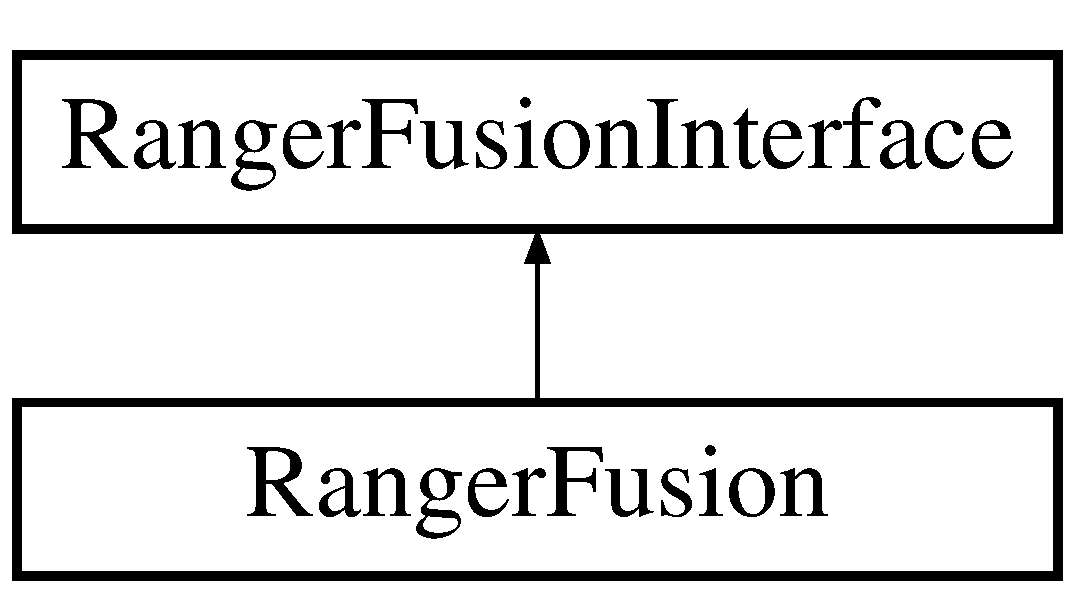
\includegraphics[height=2.000000cm]{classRangerFusionInterface}
\end{center}
\end{figure}
\subsection*{Public Member Functions}
\begin{DoxyCompactItemize}
\item 
virtual void \hyperlink{classRangerFusionInterface_aea3d7cf254c0553e624306ca06d86120}{set\+Rangers} (std\+::vector$<$ \hyperlink{classRangerInterface}{Ranger\+Interface} $\ast$ $>$ rangers)=0\hypertarget{classRangerFusionInterface_aea3d7cf254c0553e624306ca06d86120}{}\label{classRangerFusionInterface_aea3d7cf254c0553e624306ca06d86120}

\begin{DoxyCompactList}\small\item\em stores the sensor objects inside the vector \end{DoxyCompactList}\item 
virtual std\+::vector$<$ double $>$ \hyperlink{classRangerFusionInterface_a92a67e0f8f17d7bf0059002dcbeb5da8}{get\+Fused\+Range\+Data} ()=0\hypertarget{classRangerFusionInterface_a92a67e0f8f17d7bf0059002dcbeb5da8}{}\label{classRangerFusionInterface_a92a67e0f8f17d7bf0059002dcbeb5da8}

\begin{DoxyCompactList}\small\item\em returns the fused vector \end{DoxyCompactList}\item 
virtual std\+::vector$<$ std\+::vector$<$ double $>$ $>$ \hyperlink{classRangerFusionInterface_a9d60ca5866261026b870d7c0171587f5}{get\+Raw\+Range\+Data} ()=0\hypertarget{classRangerFusionInterface_a9d60ca5866261026b870d7c0171587f5}{}\label{classRangerFusionInterface_a9d60ca5866261026b870d7c0171587f5}

\begin{DoxyCompactList}\small\item\em generates the data for each sensor and the fused vectir as well \end{DoxyCompactList}\item 
virtual void \hyperlink{classRangerFusionInterface_a5eb055bfcf3ac38dd82cde5d0661e11e}{set\+Fusion\+Method} (Fusion\+Method)=0\hypertarget{classRangerFusionInterface_a5eb055bfcf3ac38dd82cde5d0661e11e}{}\label{classRangerFusionInterface_a5eb055bfcf3ac38dd82cde5d0661e11e}

\begin{DoxyCompactList}\small\item\em provides the calculations of each method of min, max and average, replaces fused vector with values depending on the method chosen \end{DoxyCompactList}\end{DoxyCompactItemize}


\subsection{Detailed Description}
\hyperlink{classRangerFusionInterface}{Ranger\+Fusion\+Interface} base class. 

This is the base class.~\newline
\begin{DoxyAuthor}{Author}
Johnsonn Nguyen 
\end{DoxyAuthor}
\begin{DoxyVersion}{Version}
1 
\end{DoxyVersion}
\begin{DoxyDate}{Date}
2019 
\end{DoxyDate}
\begin{DoxyPrecond}{Precondition}
none 
\end{DoxyPrecond}
\begin{DoxyRefDesc}{Bug}
\item[\hyperlink{bug__bug000006}{Bug}]none reported as of 2019-\/04-\/23 \end{DoxyRefDesc}
\begin{DoxyWarning}{Warning}

\end{DoxyWarning}


The documentation for this class was generated from the following files\+:\begin{DoxyCompactItemize}
\item 
/home/user/git/pfms-\/2019a-\/\+Johnson15177/scratch/assignment/a2attempt2/rangerfusioninterface.\+h\item 
/home/user/git/pfms-\/2019a-\/\+Johnson15177/scratch/assignment/a2attempt2/rangerfusioninterface.\+cpp\end{DoxyCompactItemize}

\hypertarget{classRangerInterface}{}\section{Ranger\+Interface Class Reference}
\label{classRangerInterface}\index{Ranger\+Interface@{Ranger\+Interface}}


\hyperlink{classRanger}{Ranger} interface base class.  




{\ttfamily \#include $<$rangerinterface.\+h$>$}

Inheritance diagram for Ranger\+Interface\+:\begin{figure}[H]
\begin{center}
\leavevmode
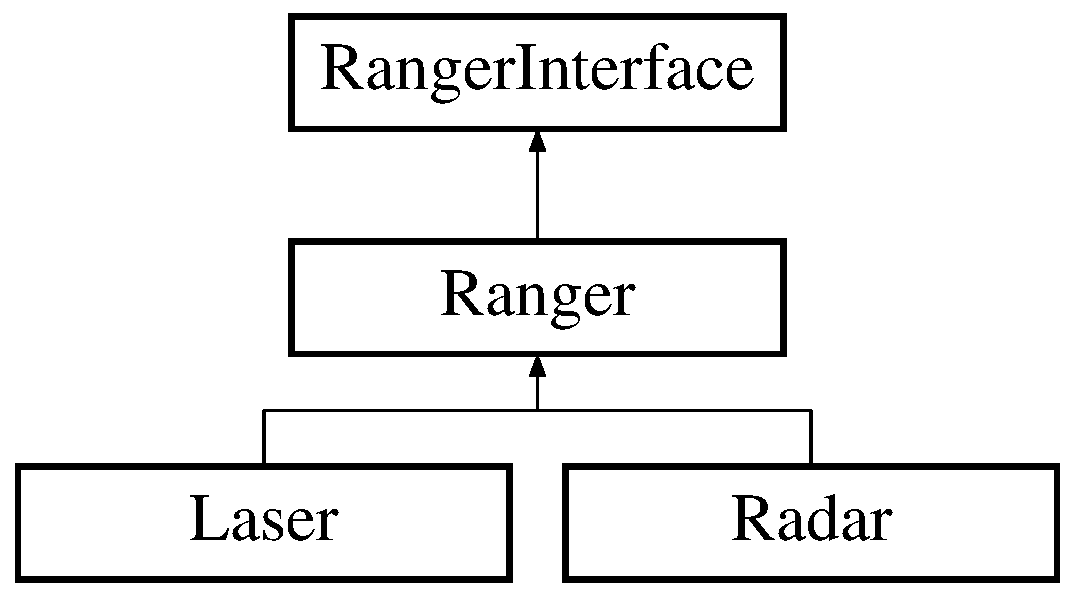
\includegraphics[height=3.000000cm]{classRangerInterface}
\end{center}
\end{figure}
\subsection*{Public Member Functions}
\begin{DoxyCompactItemize}
\item 
virtual std\+::vector$<$ double $>$ \hyperlink{classRangerInterface_a969c670cadf55a15733809116dc305c8}{generate\+Data} ()=0\hypertarget{classRangerInterface_a969c670cadf55a15733809116dc305c8}{}\label{classRangerInterface_a969c670cadf55a15733809116dc305c8}

\begin{DoxyCompactList}\small\item\em generates data for laser and radar \end{DoxyCompactList}\item 
virtual unsigned int \hyperlink{classRangerInterface_a37d4f89daffa8b2708dfc11034893552}{get\+Angular\+Resolution} (void)=0\hypertarget{classRangerInterface_a37d4f89daffa8b2708dfc11034893552}{}\label{classRangerInterface_a37d4f89daffa8b2708dfc11034893552}

\begin{DoxyCompactList}\small\item\em gets the angular resolution for laser and radar \end{DoxyCompactList}\item 
virtual int \hyperlink{classRangerInterface_a8d77cf9d9b95fe8fb315931f2f278fec}{get\+Offset} (void)=0\hypertarget{classRangerInterface_a8d77cf9d9b95fe8fb315931f2f278fec}{}\label{classRangerInterface_a8d77cf9d9b95fe8fb315931f2f278fec}

\begin{DoxyCompactList}\small\item\em gets the offset for laser and radar \end{DoxyCompactList}\item 
virtual unsigned int \hyperlink{classRangerInterface_a18716da6932402b8dda75f682be6f06c}{get\+Field\+Of\+View} (void)=0\hypertarget{classRangerInterface_a18716da6932402b8dda75f682be6f06c}{}\label{classRangerInterface_a18716da6932402b8dda75f682be6f06c}

\begin{DoxyCompactList}\small\item\em gets the field of view for laser and radar \end{DoxyCompactList}\item 
virtual double \hyperlink{classRangerInterface_a0bb29a41de5767c99081002c0590c186}{get\+Max\+Range} (void)=0\hypertarget{classRangerInterface_a0bb29a41de5767c99081002c0590c186}{}\label{classRangerInterface_a0bb29a41de5767c99081002c0590c186}

\begin{DoxyCompactList}\small\item\em gets the max range for laser and radar \end{DoxyCompactList}\item 
virtual double \hyperlink{classRangerInterface_ae6d501ddeeaad4a7b44d7d51ce64cb88}{get\+Min\+Range} (void)=0\hypertarget{classRangerInterface_ae6d501ddeeaad4a7b44d7d51ce64cb88}{}\label{classRangerInterface_ae6d501ddeeaad4a7b44d7d51ce64cb88}

\begin{DoxyCompactList}\small\item\em gets the min range for laser and radar \end{DoxyCompactList}\item 
virtual bool \hyperlink{classRangerInterface_a313296ae5d13c6acce69caaf646ea66e}{set\+Angular\+Resolution} (unsigned int)=0\hypertarget{classRangerInterface_a313296ae5d13c6acce69caaf646ea66e}{}\label{classRangerInterface_a313296ae5d13c6acce69caaf646ea66e}

\begin{DoxyCompactList}\small\item\em sets the angular resolution for laser and radar \end{DoxyCompactList}\item 
virtual bool \hyperlink{classRangerInterface_ae72584d83c94678d76f3fca20e432713}{set\+Offset} (int)=0\hypertarget{classRangerInterface_ae72584d83c94678d76f3fca20e432713}{}\label{classRangerInterface_ae72584d83c94678d76f3fca20e432713}

\begin{DoxyCompactList}\small\item\em sets the offset for laser and radar \end{DoxyCompactList}\item 
virtual bool \hyperlink{classRangerInterface_ad10f43a01e5285a654f09357028b1bb4}{set\+Field\+Of\+View} (unsigned int)=0\hypertarget{classRangerInterface_ad10f43a01e5285a654f09357028b1bb4}{}\label{classRangerInterface_ad10f43a01e5285a654f09357028b1bb4}

\begin{DoxyCompactList}\small\item\em sets the field of view for laser and radar \end{DoxyCompactList}\end{DoxyCompactItemize}


\subsection{Detailed Description}
\hyperlink{classRanger}{Ranger} interface base class. 

This is the base class for the sensors.~\newline
\begin{DoxyAuthor}{Author}
Johnsonn Nguyen 
\end{DoxyAuthor}
\begin{DoxyVersion}{Version}
1 
\end{DoxyVersion}
\begin{DoxyDate}{Date}
2019 
\end{DoxyDate}
\begin{DoxyPrecond}{Precondition}
none 
\end{DoxyPrecond}
\begin{DoxyRefDesc}{Bug}
\item[\hyperlink{bug__bug000007}{Bug}]none reported as of 2019-\/04-\/23 \end{DoxyRefDesc}
\begin{DoxyWarning}{Warning}

\end{DoxyWarning}


The documentation for this class was generated from the following files\+:\begin{DoxyCompactItemize}
\item 
/home/user/git/pfms-\/2019a-\/\+Johnson15177/scratch/assignment/a2attempt2/rangerinterface.\+h\item 
/home/user/git/pfms-\/2019a-\/\+Johnson15177/scratch/assignment/a2attempt2/rangerinterface.\+cpp\end{DoxyCompactItemize}

%--- End generated contents ---

% Index
\backmatter
\newpage
\phantomsection
\clearemptydoublepage
\addcontentsline{toc}{chapter}{Index}
\printindex

\end{document}
